\documentclass[a4paper,11pt]{paper}

\usepackage[T1]{fontenc}
\usepackage[spanish]{babel} 
\usepackage[utf8]{inputenc}
\usepackage{graphicx}
\usepackage{xcolor}
\usepackage{pdflscape}
\usepackage[breaklinks=true]{hyperref}
\usepackage{cite}

\renewcommand\familydefault{\sfdefault}
\usepackage{tgheros}
\usepackage[defaultmono]{droidmono}

\usepackage{amsmath,amssymb,amsthm,textcomp}
\usepackage{enumerate}
\usepackage{multicol}
\usepackage{tikz}
\usepackage{courier}
\usepackage{geometry}
\geometry{total={210mm,297mm},
left=25mm,right=25mm,%
bindingoffset=0mm, top=20mm,bottom=20mm}


\linespread{1.3}

\newcommand{\linia}{\rule{\linewidth}{0.5pt}}

% my own titles
\makeatletter
\renewcommand{\maketitle}{
\begin{center}
\vspace{2ex}
{\huge \textsc{\@title}}
\vspace{1ex}
\\
\linia\\
\@author \hfill \@date
\vspace{4ex}
\end{center}
}
\makeatother
%%%

% custom footers and headers
\usepackage{fancyhdr}
\pagestyle{fancy}
\lhead{}
\chead{}
\rhead{}
\lfoot{}
\cfoot{}
\rfoot{\thepage}
\renewcommand{\headrulewidth}{0pt}
\renewcommand{\footrulewidth}{0pt}
%

% code listing settings
\usepackage{listings}

\lstset{
    string=[s]{"}{"},
    stringstyle=\color{blue},
    comment=[l]{:},
    commentstyle=\color{black},
}

\begin{document}

\title{Instructivo para eliminación de estrategias}

\author{César Cárdenas | Gana+ Back-End}

\date{}
\pagenumbering{gobble}
\maketitle
\vspace*{\fill}
\begin{figure}[!h]
\centering

\includegraphics[width=0.6\textwidth]{imgs/logo.png}
\end{figure}

\begin{figure}[!h]

\includegraphics[width=0.60\textwidth]{imgs/Mongo.png}

\includegraphics[width=0.40\textwidth]{imgs/Elasticsearch.png}
\end{figure}
\vspace*{\fill}

\newpage
\tableofcontents
\newpage
\pagenumbering{arabic}


\section{Proceso de sincronización de estrategias}

\begin{figure}[!h]
  \centering
  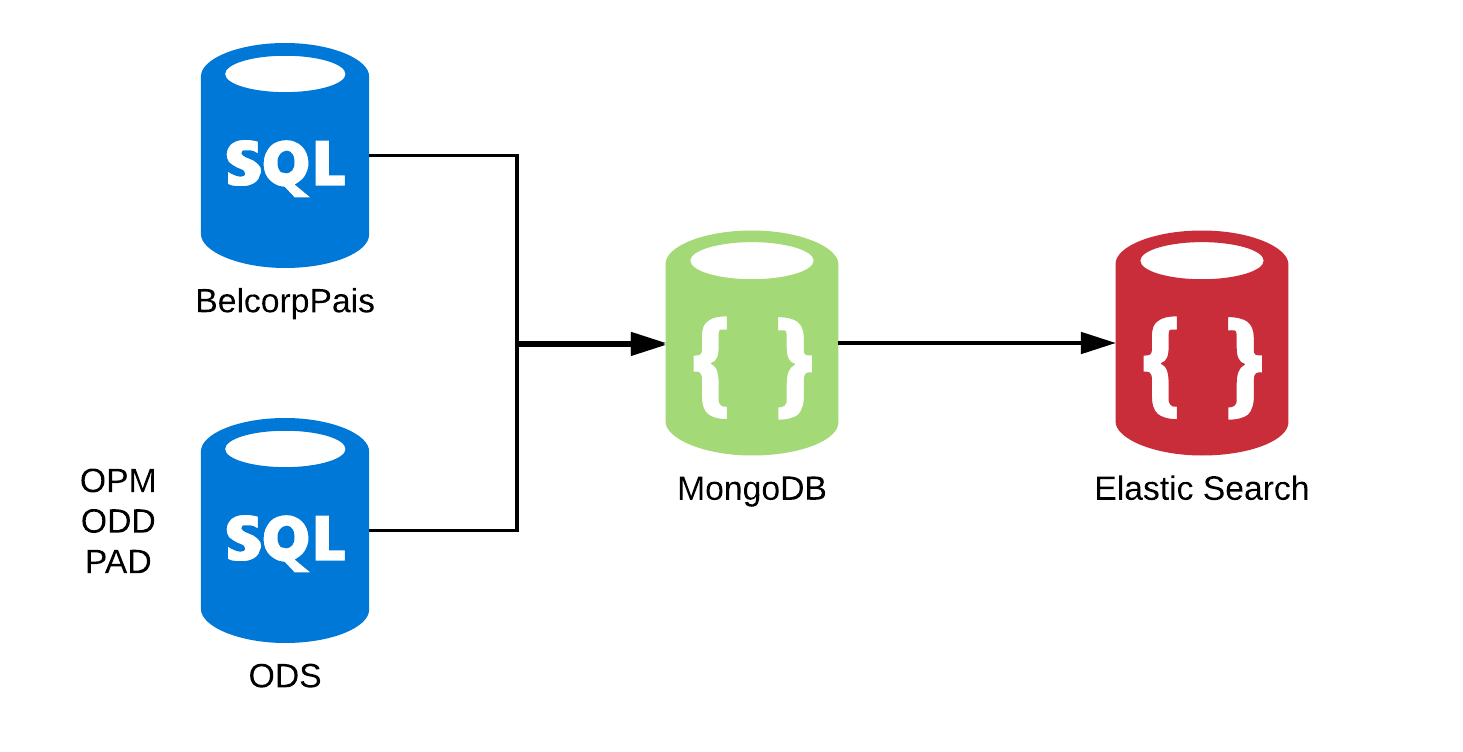
\includegraphics[width=1.0\textwidth]{imgs/FlujoEstrategias.png}
  \caption{Flujo de datos de estrategias}
  \end{figure}


\newpage
\section{Proceso de eliminación de estrategias}
\subsection{Copia de respaldo de estrategias}
\begin{enumerate}
\def\labelenumi{\arabic{enumi}.}
\item
	Ingresar a la herramienta de consultas para MongoDB (NoSQL Booster) y conectarse a la base de datos donde se elminarán las estrategias.
\item
	Consultar la estrategias que se van a eliminar, utilizando como ejemplo la siguiente sentencia
\begin{lstlisting}
db.Estrategia.find({
    TipoPersonalizacion: "ODD",
    CodigoCampania: "201813",
    CUV2: {$in: [
        "32229",
        "32230",
        "32231"
        ]}
})
\end{lstlisting}

\item
	En el visor de resultados, seleccionar la vista JSON o presionar las teclas CTRL + 3
\begin{figure}[!h]
  \centering
  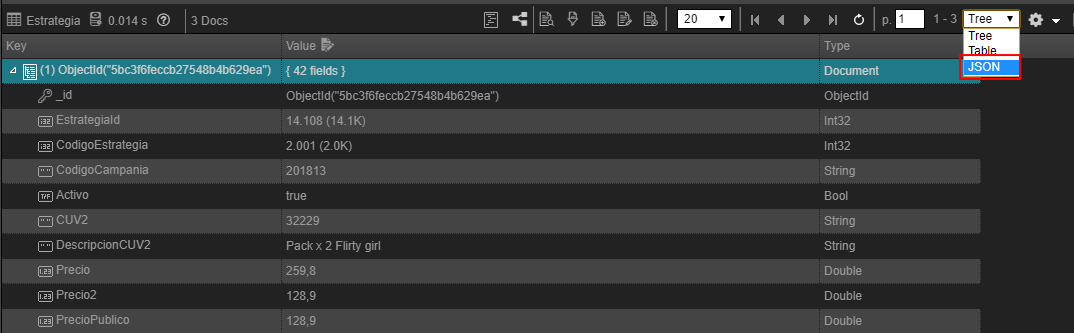
\includegraphics[width=0.9\textwidth]{imgs/ConsultaJson.png}
  \caption{Visor de resultados NoSQL Booster}
  \end{figure}

\item
	Seleccionar los registros, hacer clic derecho y seleccionar la opción Copy.
\begin{figure}[!h]
  \centering
  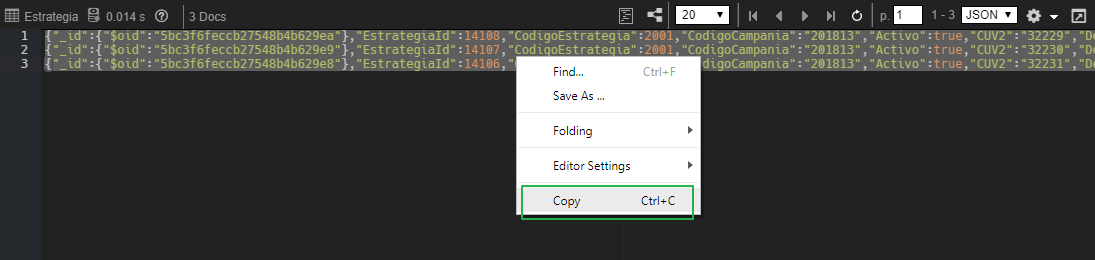
\includegraphics[width=0.9\textwidth]{imgs/CopiaResultado.png}
  \caption{Copia de registros json}
  \end{figure}

\newpage
\item
	Abrir un editor de texto con un documento en blanco y pegar los registros del paso anterior.
\item
	Guardar el archivo creado, modificando la extensión a .json
\begin{figure}[!h]
  \centering
  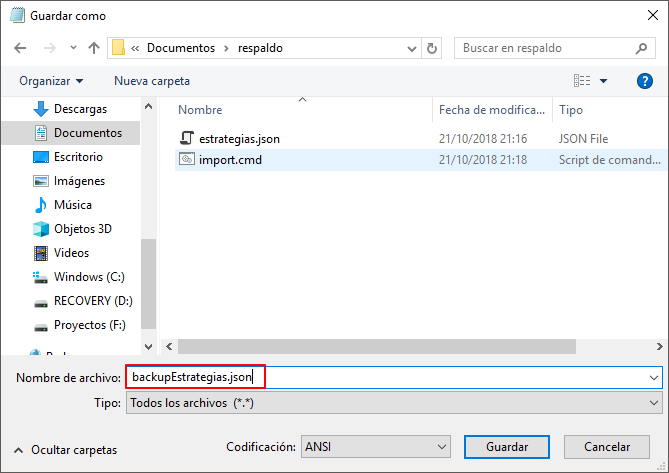
\includegraphics[width=0.9\textwidth]{imgs/GuardarArchivo.png}
  \caption{Guardar archivo json}
  \end{figure}
\end{enumerate}

Con esto, ya se tendría la copia de respaldo de las estrategias a eliminar.

\subsection{Eliminación de estrategias en MongoDB}

\begin{enumerate}
\def\labelenumi{\arabic{enumi}.}
\item
	Ingresar a la herramienta de consultas para MongoDB (NoSQL Booster) y conectarse a la base de datos donde se elminarán las estrategias.

\item
	Eliminar las estrategias, utilizando como ejemplo la siguiente sentencia
\begin{lstlisting}
db.Estrategia.remove({
    TipoPersonalizacion: "ODD",
    CodigoCampania: "201813",
    CUV2: {$in: [
        "32229",
        "32230",
        "32231"
        ]}
})
\end{lstlisting}
\newpage
\item
	Validar que las estrategias hayan sido borradas, por medio de la siguiente consulta.
\begin{lstlisting}
db.Estrategia.find({
    TipoPersonalizacion: "ODD",
    CodigoCampania: "201813",
    CUV2: {$in: [
        "32229",
        "32230",
        "32231"
        ]}
})
\end{lstlisting}


\end{enumerate}
\subsection{Eliminación de estrategias en Elastic Search}



\newpage
\section{Recuperación de estrategias eliminadas}
%\newpage
%\bibliographystyle{unsrt}
%\addcontentsline{toc}{section}{Referencias}
%\bibliography{biblio}

\end{document}
